\documentclass[a4paper,12pt]{article}
\usepackage{czech}
\usepackage[utf8]{inputenc}
\usepackage{a4wide}
\usepackage[dvipdfm]{graphicx}
\usepackage{graphics}
\usepackage{indentfirst}
\usepackage{fancyhdr}
\usepackage{setspace}
\usepackage{amsmath}
\usepackage{amssymb}
\usepackage{epsfig}

%%\usepackage{nopageno}
%%\usepackage{txfonts}
\usepackage[usenames]{color}

\begin{document}

\section{Úkol}
\begin{enumerate}
\item Ze změřeného ohybového obrazce zobrazeného na milimetrovém papíru určete mřížkovou konstantu mřížky.
\item Pomocí aparatury proměřte ohybové obrazce: mřížky, 2 vybraných štěrbin, 2 vybraných dvojštěrbin. Zpracováním měření určete parametry použitých difrakčních prvků.
\item Okalibrujte mikroskopový okulár metodou postupných měření a lineární regresí, odhadněte relativní chybu kalibrace.
\item Mikroskopem změřte parametry všech použitých difrakčních prvků.
\item Výsledky měření v úkolech č.1, č.2 a č.4 srovnejte a diskutujte, v kterém případě jsou spočtené parametry zatíženy nejmenší chybou. 
\end{enumerate}

\section{Teorie}
\subsection{Oprická mřížka}
Optická mřížka je optická součástka sloužící k ohybu světla. Tento ohyb je svázán rovnicí
\begin{eqnarray}
\sin\varphi=\frac{k\lambda}{a},
\end{eqnarray}
kde $\varphi$ je úhel pod kterým vychází kolmo dopadající paprsek, $k$ přiroené číslo a $a$ vzálenost mezi vrypy na mřížce. 
Mřížková konstanta se definuje jako převrácená hodnota $a$.

\subsection{Štěrbina a dvojstěrbina}
Dle \cite{maly} dochází na stětbinách také k ohybu. Vlivem drahových rozdílů následně vzniká na stínítku interferenční obrazec. 
Pro štěrbinu platí
\begin{eqnarray}
I=I_0\frac{\sin^2(\frac{\pi b}{\lambda}\sin\varphi)}{(\frac{\pi b}{\lambda}\sin\varphi)^2},
\label{St}
\end{eqnarray}
kde $I_0$ je maximum, které nastává pro úhel $\varphi = 0$, $b$ je šířka stěrbiny.

Pro dvojštěrbinu výraz podobný
\begin{eqnarray}
I=I_0\frac{\sin^2(\frac{\pi b}{\lambda}\varphi)}{(\frac{\pi b}{\lambda}\varphi)^2}\cos^2\left(\frac{\pi a}{\lambda}\varphi\right),
\label{DSt}
\end{eqnarray}
kde $a$ je vzdálenost středů stěrbin.

\section{Měření}
\subsection{Mřížková konstanta}
Po nastavení stínítka do ohniska čočky v aparatuře (f = 1 m) jsem na milimetrový papír zanesl ohybový obrazec vzniklý ze mnou požité mřížky. 
Odečtené hodnoty jsou vzhledem k bodu nultého řádu v tabulce \ref{TU1} včetně dopočteného průberu a odpovídající mřížkové konstantě ($\lambda = 632.8$ nm).

\begin{table}
$$
\begin{array}{|c|c|c|c|c|}
\hline
k&  x_{k1}/\mbox{mm}&  -x_{k2}/\mbox{mm}&   x_k/\mbox{mm}& a^{-1}/\mbox{mm}^{-1}  \\ \hline
1&  13.0 \pm 0.5 & 12.0 \pm 0.5&    13 \pm 1&   20\pm 2 \\ \hline
2&  25.5  \pm 0.5  & 25.0\pm 0.5&   25\pm 1&    20\pm 2 \\ \hline
3&  38.0 \pm 0.5&    37.0\pm 0.5&   38\pm 1&    20\pm 2 \\ \hline
4&  50.5 \pm 0.5&  49.0\pm 0.5& 50\pm 1&    20\pm 2 \\ \hline
5&  63.0 \pm 0.5&  62.0\pm 0.5& 63\pm 1&    20\pm 2 \\ \hline
6&  75.0 \pm 0.5&  75.0\pm 0.5& 75\pm 1&    20\pm 2 \\ \hline
7&  88.0 \pm 0.5&  87.0\pm 0.5& 88\pm 1&    20\pm 2 \\ \hline
8&  100.0 \pm 0.5& 100.0\pm 0.5&    100\pm 1&   20\pm 2 \\ \hline
9&  103.0 \pm 0.5& 103.0\pm 0.5&    103\pm 1&   18\pm 2 \\ \hline
10& 116.0\pm 0.5&  115.0\pm 0.5&    116\pm 1&   18\pm 2 \\ \hline
\end{array}
$$
\caption{Výsledky měření mřížky s pomocí milimetrového papíru.}
\label{TU1}
\end{table}

Po statistickém vyhodnocení a vypuštěním dvou posledních naměřených hodnot (z důvodu vyšší nepřesnosti při odečítání) jsem získal mřížkovou konstantu
\begin{eqnarray}
a^{-1}=(20\pm 1)\mbox{mm}^{-1}
\end{eqnarray}
Dominantní složka chyby byla nepřesnost milimetrového papíru.

Dále jsem k měření použil čidla, které jsem opět umístil do ohniska použité čočky. Data byla zanamenávána za pomoci počítače. Výsledný graf je na obrázku \ref{g1}. 
Z něj jsem za pomoci programu gnuplot odečetl maximální hodnoty a opět vyhodnotil mřížkovou konstantu. V tomto případě mi vyšlo
\begin{eqnarray}
a^{-1}=(19.24 \pm 0.02)\mbox{mm}^{-1}
\end{eqnarray}
Dle šířky píků jsem chybu odhadl na 0.1 \%.

\subsection{Stěrbina}
Čidlo jsem dále použil pro měření dvou štěrbin různé šířky. Výsledky jsou na obrázku 
\ref{g2} a \ref{g3}. Na naměřené hodnoty jsem nafitoval křivky odpovídající předpisům z rovnic \ref{St} a \ref{DSt}. Z toho jsem získal parametry štěrbin. Grafy jsou také posunuty, aby bylo maximum v bodě nula. Konkrétně rozměr štěrbin A a C
\begin{eqnarray}
b_{StA}&=&(0.1227 \pm 0.0001) \mbox{mm}\\
b_{StC}&=&(0.4514 \pm 0.0008) \mbox{mm}
\end{eqnarray}
Pro dvojštěrbiby vyšlo
\begin{eqnarray}
b_{DStA}&=&(0.1183 \pm 0.0006) \mbox{mm}\\
a_{DStA}&=&(0.6106 \pm 0.0005) \mbox{mm}\\
b_{DStC}&=&(0.2015 \pm 0.0002) \mbox{mm}\\
a_{DStC}&=&(1.2049 \pm 0.0003) \mbox{mm}
\end{eqnarray}

\subsection{Mikroskop}
Pro měření za pomoci mikroskopu se nejdříve musela provést jeho kalibrace. K tomu jsem 
použil přiloženou stupnici a odpovídající hodnoty odečtené na mikroskopu jsou v tabulce 
\ref{TMik}. Z nich jsem sestavil kalibrační křivku \ref{kal}, z které jsem stanovil velikost jednoho dílku mikroskopu
\begin{eqnarray}
d_mik=(0.1652\pm0.0005) \mbox{mm}
\end{eqnarray}
a následně naměřil rozměry zkoumaných předmětů \ref{TMH}.

\begin{table}
$$
\begin{array}{|c|c|}
\hline
x/\mbox{mm}& x/\mbox{d. mik.} \\ \hline
0.0&    0.48 \\ \hline
0.1&    1.08 \\ \hline
0.2&    1.78 \\ \hline
0.3&    2.38 \\ \hline
0.4&    2.98 \\ \hline
0.5&    3.59 \\ \hline
0.6&    4.15 \\ \hline
0.7&    4.79 \\ \hline
0.8&    5.37 \\ \hline
0.9&    5.98 \\ \hline
1.0&    6.60 \\ \hline
1.1&    7.17 \\ \hline
1.2&    7.78 \\ \hline
1.3&    8.38 \\ \hline
1.4&    9.00 \\ \hline
1.5&    9.62 \\ \hline
\end{array}
$$
\caption{Hodnoty z kalibrace mikroskopu}
\label{TMik}
\end{table}

\begin{table}
$$
\begin{array}{|l|c|c|}
\hline
&   x/\mbox{d. mik.}&   x/\mbox{mm} \\ \hline
a_{mriz}&   0.335&  0.0553 \pm 0.0002  \\ \hline
b_{StA}&    0.77&   0.127 \pm 0.001 \\ \hline
b_{StC}&    2.85&   0.471 \pm 0.001 \\ \hline
b_{DStA}&   0.76&   0.126 \pm 0.001 \\ \hline
a_{DStA}&   3.71&   0.613 \pm 0.001 \\ \hline
b_{DStC}&   1.30&   0.215 \pm 0.001 \\ \hline
a_{DStC}&   7.35&   1.214 \pm 0.001 \\ \hline
\end{array}
$$
\caption{Hodnoty naměřené mikroskopek}
\label{TMH}
\end{table}

\section{Dikuze}
Měření za pomoci milimetrového papíru se ukázalo být vcelku přesné pro stanovení 
přibližné hodnoty. Jeho chyba se však od ostatních metod lišila o celý řád. Jako 
nejpřesnější hodnotím interferenční jevy. Fitování na naměřené hodnoty sice bylo často 
zdlouhavé a zejména u dvoujštěrbiny C jsem narazil na problém s rozpoznávací schopností 
čidla. Relativní chyba je však nejmenší. U mikroskopu navíc není zcela přesně započítána 
chyba způsobená nepřesností kalibrační stupnice. Největším problémem při fitování 
za pomoci programu gnuplot byla potřeba přibližných hodnot, kolem kterých se má 
fitovat, k čemuž jsem samozřejmě použil hodnoty z měření mikroskopem. Bez těchto hodnot 
by bylo celé fitování téměř nemožné.


\section{Závěr}
Změřil jsem mřížkovou konstantu ohybové mřížky třemi metodami. Hodnoty jsou v pořadí milimetrový papír, čidlo, mikroskop.
\begin{eqnarray}
a^{-1}&=&(20\pm 1)\mbox{mm}^{-1} \\
a^{-1}&=&(19.24 \pm 0.02)\mbox{mm}^{-1} \\
a^{-1}&=&(18.03 \pm 0.07)\mbox{mm}^{-1}
\end{eqnarray}
Změřil jsem rozměry dvou různých štěrbin a to v pořadí za pomoci čidla a mikroskopem.
\begin{eqnarray}
b_{StA}&=&(0.1227 \pm 0.0001) \mbox{mm}\\
b_{StC}&=&(0.4514 \pm 0.0008) \mbox{mm}\\
b_{StA}&=&(0.127 \pm 0.001) \mbox{mm}\\
b_{StC}&=&(0.471 \pm 0.001) \mbox{mm}
\end{eqnarray}
Změřil jsem rozměry dvou různých dvojštěrbin opět dvěmi metodami.
\begin{eqnarray}
b_{DStA}&=&(0.1183 \pm 0.0006) \mbox{mm}\\
a_{DStA}&=&(0.6106 \pm 0.0005) \mbox{mm}\\
b_{DStC}&=&(0.2015 \pm 0.0002) \mbox{mm}\\
a_{DStC}&=&(1.2049 \pm 0.0003) \mbox{mm}\\
b_{DStA}&=&(0.126 \pm 0.001) \mbox{mm}\\
a_{DStA}&=&(0.613 \pm 0.001) \mbox{mm}\\
b_{DStC}&=&(0.215 \pm 0.001) \mbox{mm}\\
a_{DStC}&=&(1.214 \pm 0.001) \mbox{mm}
\end{eqnarray}
Nakalibroval jsem mikroskop. Kalibrační křivka je na obrázku \ref{kal}.

\begin{figure}
\begin{center}
% GNUPLOT: LaTeX picture with Postscript
\begingroup
  \makeatletter
  \providecommand\color[2][]{%
    \GenericError{(gnuplot) \space\space\space\@spaces}{%
      Package color not loaded in conjunction with
      terminal option `colourtext'%
    }{See the gnuplot documentation for explanation.%
    }{Either use 'blacktext' in gnuplot or load the package
      color.sty in LaTeX.}%
    \renewcommand\color[2][]{}%
  }%
  \providecommand\includegraphics[2][]{%
    \GenericError{(gnuplot) \space\space\space\@spaces}{%
      Package graphicx or graphics not loaded%
    }{See the gnuplot documentation for explanation.%
    }{The gnuplot epslatex terminal needs graphicx.sty or graphics.sty.}%
    \renewcommand\includegraphics[2][]{}%
  }%
  \providecommand\rotatebox[2]{#2}%
  \@ifundefined{ifGPcolor}{%
    \newif\ifGPcolor
    \GPcolorfalse
  }{}%
  \@ifundefined{ifGPblacktext}{%
    \newif\ifGPblacktext
    \GPblacktexttrue
  }{}%
  % define a \g@addto@macro without @ in the name:
  \let\gplgaddtomacro\g@addto@macro
  % define empty templates for all commands taking text:
  \gdef\gplbacktext{}%
  \gdef\gplfronttext{}%
  \makeatother
  \ifGPblacktext
    % no textcolor at all
    \def\colorrgb#1{}%
    \def\colorgray#1{}%
  \else
    % gray or color?
    \ifGPcolor
      \def\colorrgb#1{\color[rgb]{#1}}%
      \def\colorgray#1{\color[gray]{#1}}%
      \expandafter\def\csname LTw\endcsname{\color{white}}%
      \expandafter\def\csname LTb\endcsname{\color{black}}%
      \expandafter\def\csname LTa\endcsname{\color{black}}%
      \expandafter\def\csname LT0\endcsname{\color[rgb]{1,0,0}}%
      \expandafter\def\csname LT1\endcsname{\color[rgb]{0,1,0}}%
      \expandafter\def\csname LT2\endcsname{\color[rgb]{0,0,1}}%
      \expandafter\def\csname LT3\endcsname{\color[rgb]{1,0,1}}%
      \expandafter\def\csname LT4\endcsname{\color[rgb]{0,1,1}}%
      \expandafter\def\csname LT5\endcsname{\color[rgb]{1,1,0}}%
      \expandafter\def\csname LT6\endcsname{\color[rgb]{0,0,0}}%
      \expandafter\def\csname LT7\endcsname{\color[rgb]{1,0.3,0}}%
      \expandafter\def\csname LT8\endcsname{\color[rgb]{0.5,0.5,0.5}}%
    \else
      % gray
      \def\colorrgb#1{\color{black}}%
      \def\colorgray#1{\color[gray]{#1}}%
      \expandafter\def\csname LTw\endcsname{\color{white}}%
      \expandafter\def\csname LTb\endcsname{\color{black}}%
      \expandafter\def\csname LTa\endcsname{\color{black}}%
      \expandafter\def\csname LT0\endcsname{\color{black}}%
      \expandafter\def\csname LT1\endcsname{\color{black}}%
      \expandafter\def\csname LT2\endcsname{\color{black}}%
      \expandafter\def\csname LT3\endcsname{\color{black}}%
      \expandafter\def\csname LT4\endcsname{\color{black}}%
      \expandafter\def\csname LT5\endcsname{\color{black}}%
      \expandafter\def\csname LT6\endcsname{\color{black}}%
      \expandafter\def\csname LT7\endcsname{\color{black}}%
      \expandafter\def\csname LT8\endcsname{\color{black}}%
    \fi
  \fi
  \setlength{\unitlength}{0.0500bp}%
  \begin{picture}(7200.00,5040.00)%
    \gplgaddtomacro\gplbacktext{%
      \csname LTb\endcsname%
      \put(1210,704){\makebox(0,0)[r]{\strut{} 700}}%
      \put(1210,1074){\makebox(0,0)[r]{\strut{} 800}}%
      \put(1210,1444){\makebox(0,0)[r]{\strut{} 900}}%
      \put(1210,1814){\makebox(0,0)[r]{\strut{} 1000}}%
      \put(1210,2184){\makebox(0,0)[r]{\strut{} 1100}}%
      \put(1210,2554){\makebox(0,0)[r]{\strut{} 1200}}%
      \put(1210,2925){\makebox(0,0)[r]{\strut{} 1300}}%
      \put(1210,3295){\makebox(0,0)[r]{\strut{} 1400}}%
      \put(1210,3665){\makebox(0,0)[r]{\strut{} 1500}}%
      \put(1210,4035){\makebox(0,0)[r]{\strut{} 1600}}%
      \put(1210,4405){\makebox(0,0)[r]{\strut{} 1700}}%
      \put(1210,4775){\makebox(0,0)[r]{\strut{} 1800}}%
      \put(1342,484){\makebox(0,0){\strut{} 0}}%
      \put(2263,484){\makebox(0,0){\strut{} 0.5}}%
      \put(3184,484){\makebox(0,0){\strut{} 1}}%
      \put(4105,484){\makebox(0,0){\strut{} 1.5}}%
      \put(5027,484){\makebox(0,0){\strut{} 2}}%
      \put(5948,484){\makebox(0,0){\strut{} 2.5}}%
      \put(6869,484){\makebox(0,0){\strut{} 3}}%
      \put(308,2739){\rotatebox{-270}{\makebox(0,0){\strut{}$h$/keV$\cdot$m$^{-1}$}}}%
      \put(4105,154){\makebox(0,0){\strut{}$x$/cm}}%
    }%
    \gplgaddtomacro\gplfronttext{%
    }%
    \gplbacktext
    \put(0,0){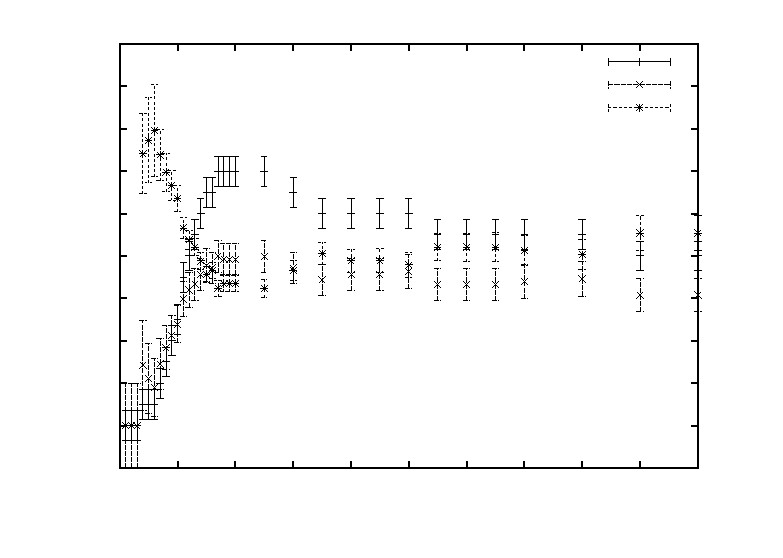
\includegraphics{g1}}%
    \gplfronttext
  \end{picture}%
\endgroup

\end{center}
\caption{Ohybový obrzec mřížky}
\label{g1}
\end{figure}

\begin{figure}
\begin{center}
% GNUPLOT: LaTeX picture with Postscript
\begingroup
  \makeatletter
  \providecommand\color[2][]{%
    \GenericError{(gnuplot) \space\space\space\@spaces}{%
      Package color not loaded in conjunction with
      terminal option `colourtext'%
    }{See the gnuplot documentation for explanation.%
    }{Either use 'blacktext' in gnuplot or load the package
      color.sty in LaTeX.}%
    \renewcommand\color[2][]{}%
  }%
  \providecommand\includegraphics[2][]{%
    \GenericError{(gnuplot) \space\space\space\@spaces}{%
      Package graphicx or graphics not loaded%
    }{See the gnuplot documentation for explanation.%
    }{The gnuplot epslatex terminal needs graphicx.sty or graphics.sty.}%
    \renewcommand\includegraphics[2][]{}%
  }%
  \providecommand\rotatebox[2]{#2}%
  \@ifundefined{ifGPcolor}{%
    \newif\ifGPcolor
    \GPcolorfalse
  }{}%
  \@ifundefined{ifGPblacktext}{%
    \newif\ifGPblacktext
    \GPblacktexttrue
  }{}%
  % define a \g@addto@macro without @ in the name:
  \let\gplgaddtomacro\g@addto@macro
  % define empty templates for all commands taking text:
  \gdef\gplbacktext{}%
  \gdef\gplfronttext{}%
  \makeatother
  \ifGPblacktext
    % no textcolor at all
    \def\colorrgb#1{}%
    \def\colorgray#1{}%
  \else
    % gray or color?
    \ifGPcolor
      \def\colorrgb#1{\color[rgb]{#1}}%
      \def\colorgray#1{\color[gray]{#1}}%
      \expandafter\def\csname LTw\endcsname{\color{white}}%
      \expandafter\def\csname LTb\endcsname{\color{black}}%
      \expandafter\def\csname LTa\endcsname{\color{black}}%
      \expandafter\def\csname LT0\endcsname{\color[rgb]{1,0,0}}%
      \expandafter\def\csname LT1\endcsname{\color[rgb]{0,1,0}}%
      \expandafter\def\csname LT2\endcsname{\color[rgb]{0,0,1}}%
      \expandafter\def\csname LT3\endcsname{\color[rgb]{1,0,1}}%
      \expandafter\def\csname LT4\endcsname{\color[rgb]{0,1,1}}%
      \expandafter\def\csname LT5\endcsname{\color[rgb]{1,1,0}}%
      \expandafter\def\csname LT6\endcsname{\color[rgb]{0,0,0}}%
      \expandafter\def\csname LT7\endcsname{\color[rgb]{1,0.3,0}}%
      \expandafter\def\csname LT8\endcsname{\color[rgb]{0.5,0.5,0.5}}%
    \else
      % gray
      \def\colorrgb#1{\color{black}}%
      \def\colorgray#1{\color[gray]{#1}}%
      \expandafter\def\csname LTw\endcsname{\color{white}}%
      \expandafter\def\csname LTb\endcsname{\color{black}}%
      \expandafter\def\csname LTa\endcsname{\color{black}}%
      \expandafter\def\csname LT0\endcsname{\color{black}}%
      \expandafter\def\csname LT1\endcsname{\color{black}}%
      \expandafter\def\csname LT2\endcsname{\color{black}}%
      \expandafter\def\csname LT3\endcsname{\color{black}}%
      \expandafter\def\csname LT4\endcsname{\color{black}}%
      \expandafter\def\csname LT5\endcsname{\color{black}}%
      \expandafter\def\csname LT6\endcsname{\color{black}}%
      \expandafter\def\csname LT7\endcsname{\color{black}}%
      \expandafter\def\csname LT8\endcsname{\color{black}}%
    \fi
  \fi
  \setlength{\unitlength}{0.0500bp}%
  \begin{picture}(7200.00,5040.00)%
    \gplgaddtomacro\gplbacktext{%
      \csname LTb\endcsname%
      \put(814,704){\makebox(0,0)[r]{\strut{} 0}}%
      \put(814,1213){\makebox(0,0)[r]{\strut{} 1}}%
      \put(814,1722){\makebox(0,0)[r]{\strut{} 2}}%
      \put(814,2231){\makebox(0,0)[r]{\strut{} 3}}%
      \put(814,2740){\makebox(0,0)[r]{\strut{} 4}}%
      \put(814,3248){\makebox(0,0)[r]{\strut{} 5}}%
      \put(814,3757){\makebox(0,0)[r]{\strut{} 6}}%
      \put(814,4266){\makebox(0,0)[r]{\strut{} 7}}%
      \put(814,4775){\makebox(0,0)[r]{\strut{} 8}}%
      \put(946,484){\makebox(0,0){\strut{} 0}}%
      \put(1404,484){\makebox(0,0){\strut{} 0.1}}%
      \put(1863,484){\makebox(0,0){\strut{} 0.2}}%
      \put(2321,484){\makebox(0,0){\strut{} 0.3}}%
      \put(2780,484){\makebox(0,0){\strut{} 0.4}}%
      \put(3238,484){\makebox(0,0){\strut{} 0.5}}%
      \put(3697,484){\makebox(0,0){\strut{} 0.6}}%
      \put(4155,484){\makebox(0,0){\strut{} 0.7}}%
      \put(4614,484){\makebox(0,0){\strut{} 0.8}}%
      \put(5072,484){\makebox(0,0){\strut{} 0.9}}%
      \put(5531,484){\makebox(0,0){\strut{} 1}}%
      \put(5989,484){\makebox(0,0){\strut{} 1.1}}%
      \put(6121,1043){\makebox(0,0)[l]{\strut{} 56}}%
      \put(6121,1722){\makebox(0,0)[l]{\strut{} 58}}%
      \put(6121,2400){\makebox(0,0)[l]{\strut{} 60}}%
      \put(6121,3079){\makebox(0,0)[l]{\strut{} 62}}%
      \put(6121,3757){\makebox(0,0)[l]{\strut{} 64}}%
      \put(6121,4436){\makebox(0,0)[l]{\strut{} 66}}%
      \put(308,2739){\rotatebox{-270}{\makebox(0,0){\strut{}$C/\mu$F}}}%
      \put(6758,2739){\rotatebox{-270}{\makebox(0,0){\strut{}$\tau/$s}}}%
      \put(3467,154){\makebox(0,0){\strut{}$I/$mA}}%
    }%
    \gplgaddtomacro\gplfronttext{%
      \csname LTb\endcsname%
      \put(5002,1317){\makebox(0,0)[r]{\strut{}$C$}}%
      \csname LTb\endcsname%
      \put(5002,1097){\makebox(0,0)[r]{\strut{}$7.72\cdot10^{-3}\{I\}$}}%
      \csname LTb\endcsname%
      \put(5002,877){\makebox(0,0)[r]{\strut{}$\tau$}}%
    }%
    \gplbacktext
    \put(0,0){\includegraphics{g2}}%
    \gplfronttext
  \end{picture}%
\endgroup

\end{center}
\caption{Graf relativní intenzity na stínítku v závislosti na poloze pro štěrbinu A.}
\label{g2}
\end{figure}

\begin{figure}
\begin{center}
% GNUPLOT: LaTeX picture with Postscript
\begingroup
  \makeatletter
  \providecommand\color[2][]{%
    \GenericError{(gnuplot) \space\space\space\@spaces}{%
      Package color not loaded in conjunction with
      terminal option `colourtext'%
    }{See the gnuplot documentation for explanation.%
    }{Either use 'blacktext' in gnuplot or load the package
      color.sty in LaTeX.}%
    \renewcommand\color[2][]{}%
  }%
  \providecommand\includegraphics[2][]{%
    \GenericError{(gnuplot) \space\space\space\@spaces}{%
      Package graphicx or graphics not loaded%
    }{See the gnuplot documentation for explanation.%
    }{The gnuplot epslatex terminal needs graphicx.sty or graphics.sty.}%
    \renewcommand\includegraphics[2][]{}%
  }%
  \providecommand\rotatebox[2]{#2}%
  \@ifundefined{ifGPcolor}{%
    \newif\ifGPcolor
    \GPcolorfalse
  }{}%
  \@ifundefined{ifGPblacktext}{%
    \newif\ifGPblacktext
    \GPblacktexttrue
  }{}%
  % define a \g@addto@macro without @ in the name:
  \let\gplgaddtomacro\g@addto@macro
  % define empty templates for all commands taking text:
  \gdef\gplbacktext{}%
  \gdef\gplfronttext{}%
  \makeatother
  \ifGPblacktext
    % no textcolor at all
    \def\colorrgb#1{}%
    \def\colorgray#1{}%
  \else
    % gray or color?
    \ifGPcolor
      \def\colorrgb#1{\color[rgb]{#1}}%
      \def\colorgray#1{\color[gray]{#1}}%
      \expandafter\def\csname LTw\endcsname{\color{white}}%
      \expandafter\def\csname LTb\endcsname{\color{black}}%
      \expandafter\def\csname LTa\endcsname{\color{black}}%
      \expandafter\def\csname LT0\endcsname{\color[rgb]{1,0,0}}%
      \expandafter\def\csname LT1\endcsname{\color[rgb]{0,1,0}}%
      \expandafter\def\csname LT2\endcsname{\color[rgb]{0,0,1}}%
      \expandafter\def\csname LT3\endcsname{\color[rgb]{1,0,1}}%
      \expandafter\def\csname LT4\endcsname{\color[rgb]{0,1,1}}%
      \expandafter\def\csname LT5\endcsname{\color[rgb]{1,1,0}}%
      \expandafter\def\csname LT6\endcsname{\color[rgb]{0,0,0}}%
      \expandafter\def\csname LT7\endcsname{\color[rgb]{1,0.3,0}}%
      \expandafter\def\csname LT8\endcsname{\color[rgb]{0.5,0.5,0.5}}%
    \else
      % gray
      \def\colorrgb#1{\color{black}}%
      \def\colorgray#1{\color[gray]{#1}}%
      \expandafter\def\csname LTw\endcsname{\color{white}}%
      \expandafter\def\csname LTb\endcsname{\color{black}}%
      \expandafter\def\csname LTa\endcsname{\color{black}}%
      \expandafter\def\csname LT0\endcsname{\color{black}}%
      \expandafter\def\csname LT1\endcsname{\color{black}}%
      \expandafter\def\csname LT2\endcsname{\color{black}}%
      \expandafter\def\csname LT3\endcsname{\color{black}}%
      \expandafter\def\csname LT4\endcsname{\color{black}}%
      \expandafter\def\csname LT5\endcsname{\color{black}}%
      \expandafter\def\csname LT6\endcsname{\color{black}}%
      \expandafter\def\csname LT7\endcsname{\color{black}}%
      \expandafter\def\csname LT8\endcsname{\color{black}}%
    \fi
  \fi
  \setlength{\unitlength}{0.0500bp}%
  \begin{picture}(7200.00,5040.00)%
    \gplgaddtomacro\gplbacktext{%
      \csname LTb\endcsname%
      \put(1210,704){\makebox(0,0)[r]{\strut{} 0}}%
      \put(1210,1382){\makebox(0,0)[r]{\strut{} 500}}%
      \put(1210,2061){\makebox(0,0)[r]{\strut{} 1000}}%
      \put(1210,2739){\makebox(0,0)[r]{\strut{} 1500}}%
      \put(1210,3418){\makebox(0,0)[r]{\strut{} 2000}}%
      \put(1210,4096){\makebox(0,0)[r]{\strut{} 2500}}%
      \put(1210,4775){\makebox(0,0)[r]{\strut{} 3000}}%
      \put(1342,484){\makebox(0,0){\strut{} 30}}%
      \put(1956,484){\makebox(0,0){\strut{} 40}}%
      \put(2570,484){\makebox(0,0){\strut{} 50}}%
      \put(3184,484){\makebox(0,0){\strut{} 60}}%
      \put(3798,484){\makebox(0,0){\strut{} 70}}%
      \put(4413,484){\makebox(0,0){\strut{} 80}}%
      \put(5027,484){\makebox(0,0){\strut{} 90}}%
      \put(5641,484){\makebox(0,0){\strut{} 100}}%
      \put(6255,484){\makebox(0,0){\strut{} 110}}%
      \put(6869,484){\makebox(0,0){\strut{} 120}}%
      \put(308,2739){\rotatebox{-270}{\makebox(0,0){\strut{}$f$/Hz}}}%
      \put(4105,154){\makebox(0,0){\strut{}$U_0$/V}}%
    }%
    \gplgaddtomacro\gplfronttext{%
    }%
    \gplbacktext
    \put(0,0){\includegraphics{g3}}%
    \gplfronttext
  \end{picture}%
\endgroup

\end{center}
\caption{Graf relativní intenzity na stínítku v závislosti na poloze pro štěrbinu C.}
\label{g3}
\end{figure}

\begin{figure}
\begin{center}
% GNUPLOT: LaTeX picture with Postscript
\begingroup
  \makeatletter
  \providecommand\color[2][]{%
    \GenericError{(gnuplot) \space\space\space\@spaces}{%
      Package color not loaded in conjunction with
      terminal option `colourtext'%
    }{See the gnuplot documentation for explanation.%
    }{Either use 'blacktext' in gnuplot or load the package
      color.sty in LaTeX.}%
    \renewcommand\color[2][]{}%
  }%
  \providecommand\includegraphics[2][]{%
    \GenericError{(gnuplot) \space\space\space\@spaces}{%
      Package graphicx or graphics not loaded%
    }{See the gnuplot documentation for explanation.%
    }{The gnuplot epslatex terminal needs graphicx.sty or graphics.sty.}%
    \renewcommand\includegraphics[2][]{}%
  }%
  \providecommand\rotatebox[2]{#2}%
  \@ifundefined{ifGPcolor}{%
    \newif\ifGPcolor
    \GPcolorfalse
  }{}%
  \@ifundefined{ifGPblacktext}{%
    \newif\ifGPblacktext
    \GPblacktexttrue
  }{}%
  % define a \g@addto@macro without @ in the name:
  \let\gplgaddtomacro\g@addto@macro
  % define empty templates for all commands taking text:
  \gdef\gplbacktext{}%
  \gdef\gplfronttext{}%
  \makeatother
  \ifGPblacktext
    % no textcolor at all
    \def\colorrgb#1{}%
    \def\colorgray#1{}%
  \else
    % gray or color?
    \ifGPcolor
      \def\colorrgb#1{\color[rgb]{#1}}%
      \def\colorgray#1{\color[gray]{#1}}%
      \expandafter\def\csname LTw\endcsname{\color{white}}%
      \expandafter\def\csname LTb\endcsname{\color{black}}%
      \expandafter\def\csname LTa\endcsname{\color{black}}%
      \expandafter\def\csname LT0\endcsname{\color[rgb]{1,0,0}}%
      \expandafter\def\csname LT1\endcsname{\color[rgb]{0,1,0}}%
      \expandafter\def\csname LT2\endcsname{\color[rgb]{0,0,1}}%
      \expandafter\def\csname LT3\endcsname{\color[rgb]{1,0,1}}%
      \expandafter\def\csname LT4\endcsname{\color[rgb]{0,1,1}}%
      \expandafter\def\csname LT5\endcsname{\color[rgb]{1,1,0}}%
      \expandafter\def\csname LT6\endcsname{\color[rgb]{0,0,0}}%
      \expandafter\def\csname LT7\endcsname{\color[rgb]{1,0.3,0}}%
      \expandafter\def\csname LT8\endcsname{\color[rgb]{0.5,0.5,0.5}}%
    \else
      % gray
      \def\colorrgb#1{\color{black}}%
      \def\colorgray#1{\color[gray]{#1}}%
      \expandafter\def\csname LTw\endcsname{\color{white}}%
      \expandafter\def\csname LTb\endcsname{\color{black}}%
      \expandafter\def\csname LTa\endcsname{\color{black}}%
      \expandafter\def\csname LT0\endcsname{\color{black}}%
      \expandafter\def\csname LT1\endcsname{\color{black}}%
      \expandafter\def\csname LT2\endcsname{\color{black}}%
      \expandafter\def\csname LT3\endcsname{\color{black}}%
      \expandafter\def\csname LT4\endcsname{\color{black}}%
      \expandafter\def\csname LT5\endcsname{\color{black}}%
      \expandafter\def\csname LT6\endcsname{\color{black}}%
      \expandafter\def\csname LT7\endcsname{\color{black}}%
      \expandafter\def\csname LT8\endcsname{\color{black}}%
    \fi
  \fi
  \setlength{\unitlength}{0.0500bp}%
  \begin{picture}(7200.00,5040.00)%
    \gplgaddtomacro\gplbacktext{%
      \csname LTb\endcsname%
      \put(1210,704){\makebox(0,0)[r]{\strut{} 900}}%
      \put(1210,1383){\makebox(0,0)[r]{\strut{} 950}}%
      \put(1210,2061){\makebox(0,0)[r]{\strut{} 1000}}%
      \put(1210,2740){\makebox(0,0)[r]{\strut{} 1050}}%
      \put(1210,3418){\makebox(0,0)[r]{\strut{} 1100}}%
      \put(1210,4097){\makebox(0,0)[r]{\strut{} 1150}}%
      \put(1210,4775){\makebox(0,0)[r]{\strut{} 1200}}%
      \put(1342,484){\makebox(0,0){\strut{} 2}}%
      \put(2263,484){\makebox(0,0){\strut{} 3}}%
      \put(3184,484){\makebox(0,0){\strut{} 4}}%
      \put(4105,484){\makebox(0,0){\strut{} 5}}%
      \put(5027,484){\makebox(0,0){\strut{} 6}}%
      \put(5948,484){\makebox(0,0){\strut{} 7}}%
      \put(6869,484){\makebox(0,0){\strut{} 8}}%
      \put(308,2739){\rotatebox{-270}{\makebox(0,0){\strut{}$H$/Am$^-1$}}}%
      \put(4105,154){\makebox(0,0){\strut{}$x$/cm}}%
    }%
    \gplgaddtomacro\gplfronttext{%
      \csname LTb\endcsname%
      \put(5882,4602){\makebox(0,0)[r]{\strut{}teoretická}}%
      \csname LTb\endcsname%
      \put(5882,4382){\makebox(0,0)[r]{\strut{}fitovaná}}%
    }%
    \gplbacktext
    \put(0,0){\includegraphics{g4}}%
    \gplfronttext
  \end{picture}%
\endgroup

\end{center}
\caption{Graf relativní intenzity na stínítku v závislosti na poloze pro dvojštěrbinu A.}
\label{g4}
\end{figure}

\begin{figure}
\begin{center}
\input{g5.tex}
\end{center}
\caption{Graf relativní intenzity na stínítku v závislosti na poloze pro dvojštěrbinu C.}
\label{g5}
\end{figure}

\begin{figure}
\begin{center}
% GNUPLOT: LaTeX picture with Postscript
\begingroup
  \makeatletter
  \providecommand\color[2][]{%
    \GenericError{(gnuplot) \space\space\space\@spaces}{%
      Package color not loaded in conjunction with
      terminal option `colourtext'%
    }{See the gnuplot documentation for explanation.%
    }{Either use 'blacktext' in gnuplot or load the package
      color.sty in LaTeX.}%
    \renewcommand\color[2][]{}%
  }%
  \providecommand\includegraphics[2][]{%
    \GenericError{(gnuplot) \space\space\space\@spaces}{%
      Package graphicx or graphics not loaded%
    }{See the gnuplot documentation for explanation.%
    }{The gnuplot epslatex terminal needs graphicx.sty or graphics.sty.}%
    \renewcommand\includegraphics[2][]{}%
  }%
  \providecommand\rotatebox[2]{#2}%
  \@ifundefined{ifGPcolor}{%
    \newif\ifGPcolor
    \GPcolorfalse
  }{}%
  \@ifundefined{ifGPblacktext}{%
    \newif\ifGPblacktext
    \GPblacktexttrue
  }{}%
  % define a \g@addto@macro without @ in the name:
  \let\gplgaddtomacro\g@addto@macro
  % define empty templates for all commands taking text:
  \gdef\gplbacktext{}%
  \gdef\gplfronttext{}%
  \makeatother
  \ifGPblacktext
    % no textcolor at all
    \def\colorrgb#1{}%
    \def\colorgray#1{}%
  \else
    % gray or color?
    \ifGPcolor
      \def\colorrgb#1{\color[rgb]{#1}}%
      \def\colorgray#1{\color[gray]{#1}}%
      \expandafter\def\csname LTw\endcsname{\color{white}}%
      \expandafter\def\csname LTb\endcsname{\color{black}}%
      \expandafter\def\csname LTa\endcsname{\color{black}}%
      \expandafter\def\csname LT0\endcsname{\color[rgb]{1,0,0}}%
      \expandafter\def\csname LT1\endcsname{\color[rgb]{0,1,0}}%
      \expandafter\def\csname LT2\endcsname{\color[rgb]{0,0,1}}%
      \expandafter\def\csname LT3\endcsname{\color[rgb]{1,0,1}}%
      \expandafter\def\csname LT4\endcsname{\color[rgb]{0,1,1}}%
      \expandafter\def\csname LT5\endcsname{\color[rgb]{1,1,0}}%
      \expandafter\def\csname LT6\endcsname{\color[rgb]{0,0,0}}%
      \expandafter\def\csname LT7\endcsname{\color[rgb]{1,0.3,0}}%
      \expandafter\def\csname LT8\endcsname{\color[rgb]{0.5,0.5,0.5}}%
    \else
      % gray
      \def\colorrgb#1{\color{black}}%
      \def\colorgray#1{\color[gray]{#1}}%
      \expandafter\def\csname LTw\endcsname{\color{white}}%
      \expandafter\def\csname LTb\endcsname{\color{black}}%
      \expandafter\def\csname LTa\endcsname{\color{black}}%
      \expandafter\def\csname LT0\endcsname{\color{black}}%
      \expandafter\def\csname LT1\endcsname{\color{black}}%
      \expandafter\def\csname LT2\endcsname{\color{black}}%
      \expandafter\def\csname LT3\endcsname{\color{black}}%
      \expandafter\def\csname LT4\endcsname{\color{black}}%
      \expandafter\def\csname LT5\endcsname{\color{black}}%
      \expandafter\def\csname LT6\endcsname{\color{black}}%
      \expandafter\def\csname LT7\endcsname{\color{black}}%
      \expandafter\def\csname LT8\endcsname{\color{black}}%
    \fi
  \fi
  \setlength{\unitlength}{0.0500bp}%
  \begin{picture}(7200.00,5040.00)%
    \gplgaddtomacro\gplbacktext{%
      \csname LTb\endcsname%
      \put(1210,704){\makebox(0,0)[r]{\strut{} 3000}}%
      \put(1210,1518){\makebox(0,0)[r]{\strut{} 3500}}%
      \put(1210,2332){\makebox(0,0)[r]{\strut{} 4000}}%
      \put(1210,3147){\makebox(0,0)[r]{\strut{} 4500}}%
      \put(1210,3961){\makebox(0,0)[r]{\strut{} 5000}}%
      \put(1210,4775){\makebox(0,0)[r]{\strut{} 5500}}%
      \put(1505,484){\makebox(0,0){\strut{} 26}}%
      \put(2155,484){\makebox(0,0){\strut{} 28}}%
      \put(2805,484){\makebox(0,0){\strut{} 30}}%
      \put(3455,484){\makebox(0,0){\strut{} 32}}%
      \put(4106,484){\makebox(0,0){\strut{} 34}}%
      \put(4756,484){\makebox(0,0){\strut{} 36}}%
      \put(5406,484){\makebox(0,0){\strut{} 38}}%
      \put(6056,484){\makebox(0,0){\strut{} 40}}%
      \put(6706,484){\makebox(0,0){\strut{} 42}}%
      \put(308,2739){\rotatebox{-270}{\makebox(0,0){\strut{}$\sqrt{\omega}$}}}%
      \put(4105,154){\makebox(0,0){\strut{}Z}}%
    }%
    \gplgaddtomacro\gplfronttext{%
    }%
    \gplbacktext
    \put(0,0){\includegraphics{kal}}%
    \gplfronttext
  \end{picture}%
\endgroup

\end{center}
\caption{Kalibrační křivka mikroskopu.}
\label{kal}
\end{figure}


\eject
\begin{thebibliography}{5}
	\bibitem{text} \textbf{Studijní text na praktikum III} \\http://physics.mff.cuni.cz/vyuka/zfp/txt\_306.htm (8. 3. 2012)
    \bibitem{chyba} \emph{J. Englich}: \textbf{Zpracování výsldků fyzikálních měření} \\ LS 1999/2000
    \bibitem{maly} \emph{prof. RNDr. Petr Malý , DrSc.}: \textbf{Optika}\\Univerzita Karlova v Praze, Nakladatelství Karolinum 2008, první vydání
\end{thebibliography}



\end{document}
